
\section{The LR Circuit}

\makelabheader %(Space for student name, etc., defined in master.tex)

\textbf{Objective} 

To investigate the relationships among the voltages in a series LR
circuit.

\textbf{Apparatus} 

\begin{itemize}
\item DataStudio 750 Interface
\item AC/DC Electronics Laboratory
\item Resistor (5$\Omega$)
\item Inductor and iron core 
\item Voltage sensors (2)
\item Digital multimeter (DMM)
\item LR Circuit activity
\item Wires to complete the circuit
\end{itemize}
\textbf{Introduction} 

In this exercise you will study a series LR circuit. If a sinusoidally
varying source of emf with a frequency f is placed in series with
a resistor and a pure inductor, the current $I$ will vary with the same
frequency as the generator, but it will be shifted in phase by an
angle \( \phi  \) relative to the voltage of the generator. The voltage
across each of the circuit elements has its own characteristic phase
relationship with the current. The voltage across the resistor V\( _{R} \)
is in phase with the current $I$, the voltage across the inductor V\( _{L} \)
leads the current by 90\( ^{\circ } \), and the voltage across the
generator leads the current by the phase angle \( \phi  \) whose
value is dependent on the circuit parameters. Measurements of the
voltage across each element in a series circuit containing an inductor,
a resistor, and a sine wave generator will be used to perform a detailed
study of the LR circuit.

\vspace{0.3cm}
{\centering \resizebox*{0.75\textwidth}{!}{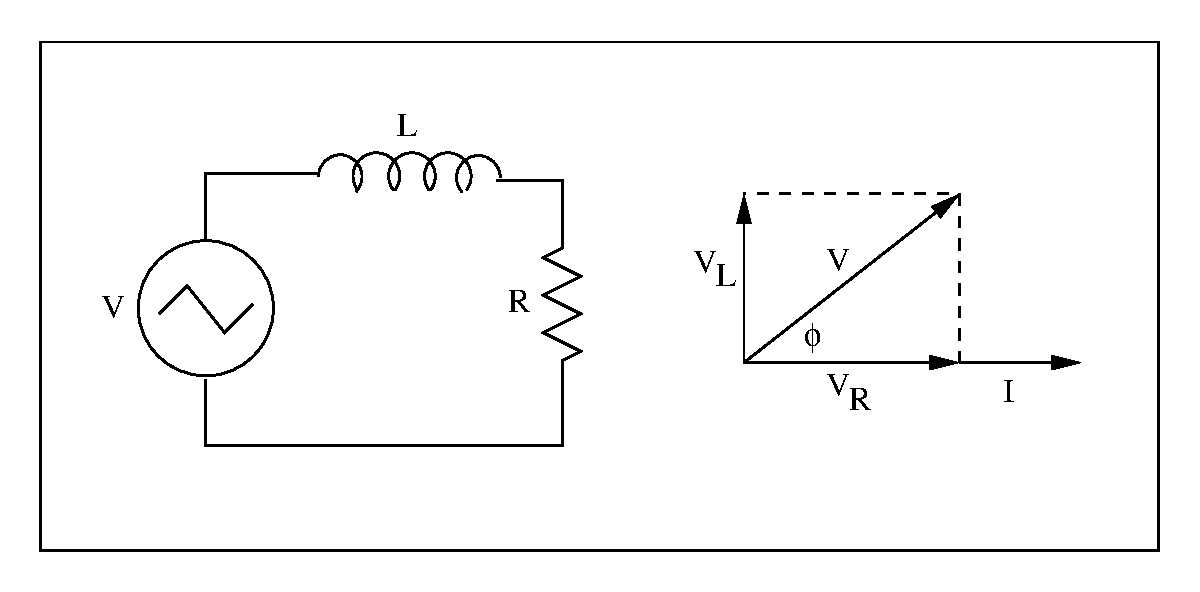
\includegraphics{lr_circuit/lr_circuit_fig_1.eps}} \par}
\vspace{0.3cm}

Let's begin by considering the circuit obtained by placing a pure
inductance $L$ and a resistor $R$ in series with a sine wave generator
with a voltage amplitude V as shown in the figure above. Also shown
in the figure is a phasor diagram for the circuit. Note that the voltage
across the resistor V\( _{R} \) is in phase with the current $I$, the
voltage across the inductor V\( _{L} \) is 90\( ^{\circ } \) ahead
of $I$, and the generator voltage V is angle \( \phi  \) ahead of $I$.
From the phasor diagram we can write 

\[
V=\sqrt{V_{L}^{2}+V_{R}^{2}}\]


and 

\[
\tan \phi =\frac{V_{L}}{V_{R}}=\frac{I\omega L}{IR}=\frac{\omega L}{R}\]


where \( \omega  \) =2\( \pi  \)f is the angular frequency of
the generator and we have used the inductive reactance and Ohm's Law.

Real inductors have both an inductance $L$ and an internal resistance
$r$. A real inductor can be represented by a pure inductance $L$ in series
with a resistance $r$. In the figure below a real inductor is shown
in series with a resistor $R$ and a generator of voltage amplitude V.
Also shown in the figure is a phasor diagram for the circuit. The
voltage across the real inductor is referred to as V\( _{ind} \).
There is, of course, some voltage V\( _{L} \) across $L$ alone, and
some voltage V\( _{r} \) across $r$ alone. However, there can be no
direct measurement of V\( _{L} \) or V\( _{r} \) since they are from the
same length of wire. The only quantity
which can be measured is V\( _{ind} \) which is the vector sum of
V\( _{L} \) and V\( _{r} \). Applying the law of cosines to the
triangle formed by V, V\( _{R} \), and V\( _{ind} \) leads to the
following equation.

\[
V_{ind}^{2}=V^{2}+V_{R}^{2}-2VV_{R}\cos \phi \]


Solving this equation for cos \( \phi  \) we get

\[
\cos \phi =\frac{V^{2}+V_{R}^{2}-V_{ind}^{2}}{2VV_{R}}\]


Further examination of the phasor diagram shows that the unknown voltages
V\( _{L} \) and V\( _{r} \) can be determined from V, V\( _{R} \),
and \( \phi  \) by the following: 

{\centering \( V_{L}=V\sin \phi  \) \par}

{\centering \( V_{r}=V\cos \phi -V_{R} \)\par}

The current $I$ can be related to the voltage across each element by
the following equations:

\[
V_{L}=I\omega L\]


\[
V_{R}=IR\]


%\[
%V_{r}=Ir\]


Once V\( _{L} \) and V\( _{r} \) have been determined, the equations
above can be used to solve for \( \omega  \)L by eliminating
$I$ to get 

{\centering \( \omega L=R\frac{V_{L}}{V_{R}} \) \par}

%{\centering \( r=R\frac{V_{r}}{V_{R}} \)\par}

\vspace{0.3cm}
{\centering \resizebox*{0.75\textwidth}{!}{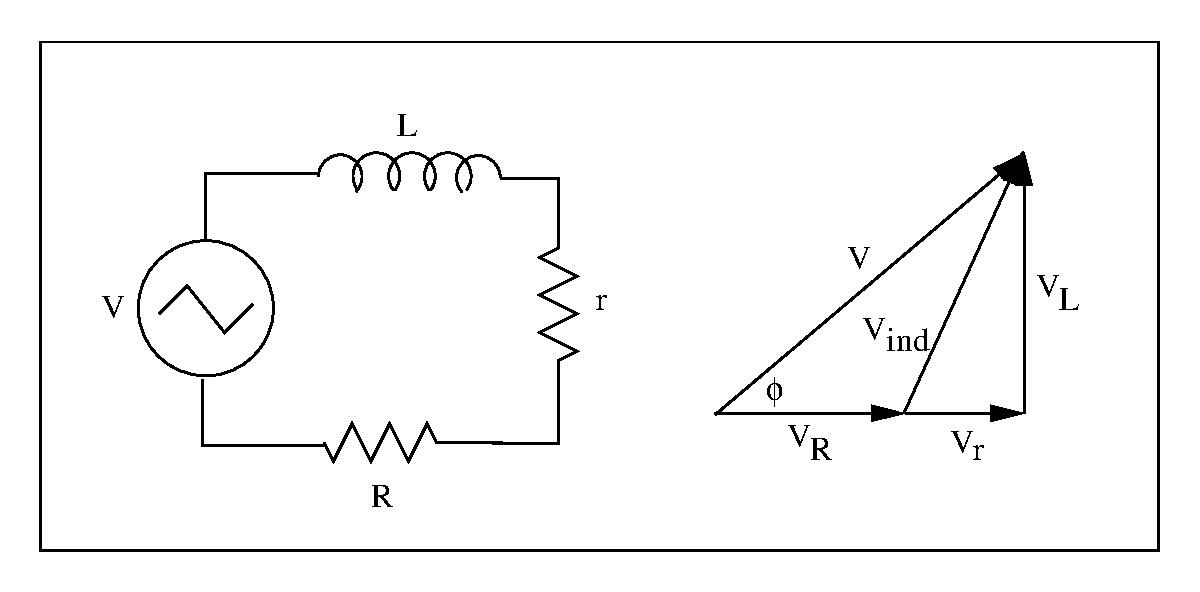
\includegraphics{lr_circuit/lr_circuit_fig_2.eps}} \par}
\vspace{0.3cm}

\textbf{Activity 1: Voltage in the LR Circuit }

In this laboratory you will be using a voltage source that varies
sinusoidally in time.
What will the voltage from this source look like as a function
of time?
In the space below sketch your answer.
What is the phase relationship between the source voltage and the
voltage drop across an inductor?
Sketch that relationship on the same graph below.
Label your curve $V_{ind}$.
What is the phase relationship between the voltage drop
across a resistor in the LR circuit and the source voltage?
Sketch it below and label it $V_R$.

\vspace{0.3cm}
{\centering \resizebox*{0.75\textwidth}{!}{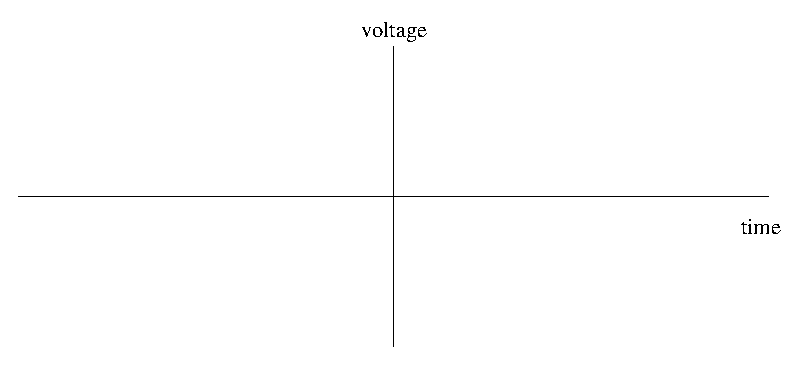
\includegraphics{lr_circuit/lr_circuit_fig_3.eps}} \par}
\vspace{0.3cm}

\textbf{Activity 2: Measuring Voltages} 

(a) Construct a data table with 2 columns and nine rows in the space
below. In the first column, label the rows $R$ (\( \Omega  \)), $r$ (\( \Omega  \)), V (V),
V\( _{R} \) (V), V\( _{ind} \) (V), \( \phi  \) (deg), V\( _{L} \)
(V), V\( _{r} \) (V), and $L$ (H).
\vspace{4in}

(b) Open the \emph{LR Circuit} activity
in the 132 Workshop folder in the Programs menu. 
Go to the `Signal Generator' window and set the frequency to 50 Hz, the amplitude 
to 3.0 V, and the wave form to `Sine Wave'.
If you can't find the `Signal Generator' window, click the `setup' button at
the top of the DataStudio menu.
You will see an image of the Pasco 750 interface with several
connections marked.
Single click on the one called `Output'.
The `Signal Generator' window should pop up. 
Set the values on it and return to the original voltage graph window.

(c) Set up the circuit on the AC/DC Electronics Laboratory so that it corresponds to the one shown in the second figure. The iron core (a long metal cylinder) should be inserted in the inductor. The inductor is the large open, cylinder in the upper-right-hand part of the AC/DC Electronics Laboratory.
The computer is set up to measure the voltage
across each of the circuit elements. The resistor in the circuit 
has a value $R\approx 5\Omega$. Check this value with the DMM and record it
as $R$ on your data sheet. Measure and record the value for $r$ with the DMM.
\textbf{NOTE: These values must be measured with $R$ and $L$ disconnected from the circuit.}

(d) Take data by clicking the \emph{Start} button. The computer will display three sinusoidal
voltage signals. The color scheme to identify each voltage measurement
is shown on the right of the voltage graph window. Determine which trace
corresponds to V (the source signal), V\( _{R} \) (the resistor voltage), and V\( _{ind} \) (the inductor voltage). 
Print a copy of this graph and attach it to this unit.
Check that the phase relationships agree with
the phasor diagram in the second figure above, i.e. V\( _{ind} \) leads V, V\( _{R} \) lags V.
\vspace{5.0mm}

\hspace{2.0in} V\( _{ind} \) leads V?
\vspace{5.0mm}

\hspace{2.0in} V\( _{R} \) lags V?
\vspace{5.0mm}

(e) Measure the amplitude of each of the signals and record these
quantities in your data table. This can be done using the SmartTool 
(see Appendix \ref{datastudio}), or read directly from the graph.

\textbf{Activity 3: Analyzing the Circuit}
 
(a) Calculate the remaining quantities necessary to complete your
data table. Show the calculations in the space below.
\vspace{3in}

(b) Determine and record the  value of $L$  for your inductor.
Make careful note of
the particular inductor and AC/DC Electronics Laboratory
which you have used. You may need to identify
it and use it again in another laboratory exercise.
\vspace{1.5in}

\newpage

(c) Construct to scale a phasor diagram like the one shown in the
second figure in the space below, based on your data.
\vspace{2in}

%(d) If your inductor was used in a series circuit with a 10-k\( \Omega  \)
%resistor and a generator with f = 20 kHz, what would be the phase
%angle \( \phi  \)?

(d) From the three sinusoidal voltage signals found in 2(d) above, determine the phase difference between the resistor voltage and the output voltage, convert to degrees and compare with your calculated value of \( \phi  \). You may want to expand the time axis on the graph to do this more accurately. Also, determine the phase difference between the resistor voltage and the inductor voltage, convert to degrees and compare with the corresponding angle in your phasor diagram above. Present the results here.
\vspace{1.2in}

\textbf{Activity 4: Determining L from Half-life Measurement}

(a) Delete the sinusoidal graphs from Activity 2.

(b) Go to the 'Signal Generator' window and change the wave form to 'Positive Square Wave' and the frequency to 30 Hz. 

(c) Take data by clicking the \emph{Start} button. The computer will display a square wave for the output voltage, and rising and falling exponential curves for the voltages across the resistor and inductor, characteristic of an LR circuit energized by a constant emf.

(d) Measure the half-life from one of the exponential curves.
\vspace{10mm}

(e) Determine the time constant \( \tau  \) from \( \tau  \) = half-life/ln2.
\vspace{10mm}

(f) Determine the inductance $L$ from \( \tau  \) = $L/R$.
\vspace{15mm}

Does the result agree with what you found in Activity 3? What is the percent difference?




